\documentclass[11pt]{article}
\usepackage[margin=1in]{geometry}
\usepackage{amsmath,amssymb,amsfonts}
\usepackage{tikz}
\usetikzlibrary{arrows.meta,positioning,calc,decorations.pathreplacing,fit,backgrounds}
\usepackage{algorithm}
\usepackage{algpseudocode}
\usepackage{booktabs}
\usepackage{xcolor}
\usepackage{hyperref}

\definecolor{trevblue}{RGB}{41,98,255}
\definecolor{trevred}{RGB}{220,50,50}
\definecolor{trevgreen}{RGB}{0,150,80}
\definecolor{trevorange}{RGB}{240,140,0}
\definecolor{lightgray}{RGB}{240,240,240}

\title{\textbf{Gradient Methods for Tensor Ring VQE}\\[4pt]
\large Parameter-Shift vs Autograd (Backpropagation)}
\author{TREV Documentation}
\date{}

\begin{document}
\maketitle

%=============================================
\section{Overview}

Given a parameterized tensor ring circuit $|\psi(\boldsymbol{\theta})\rangle$ and Hamiltonian $H$, we want:
\[
\nabla_{\boldsymbol{\theta}} \langle \psi(\boldsymbol{\theta}) | H | \psi(\boldsymbol{\theta}) \rangle
\]
Two methods compute this gradient:

\begin{center}
\begin{tabular}{lcc}
\toprule
& \textbf{Parameter-Shift} & \textbf{Autograd (Backprop)} \\
\midrule
Evaluations & $2P$ (forward only) & $1$ forward + $1$ backward \\
Batching & $B$ circuits in parallel & Single circuit \\
Precision & float32 & float32 (or float64) \\
SVD backward & Not needed & Custom (F/G split) \\
\bottomrule
\end{tabular}
\end{center}

%=============================================
\section{Parameter-Shift Rule}

\subsection{Principle}
For each parameter $\theta_k$, evaluate the expectation value at two shifted points:
\[
\frac{\partial f}{\partial \theta_k} = \frac{f(\theta_k + s) - f(\theta_k - s)}{2\sin(s)}
\]
where $s = \pi/2$ for standard quantum gates. This requires \textbf{$2P$ circuit evaluations} for $P$ parameters.

\subsection{Batched Execution}

The key optimization: evaluate $B$ shifted circuits \textbf{simultaneously} on the GPU.

\begin{center}
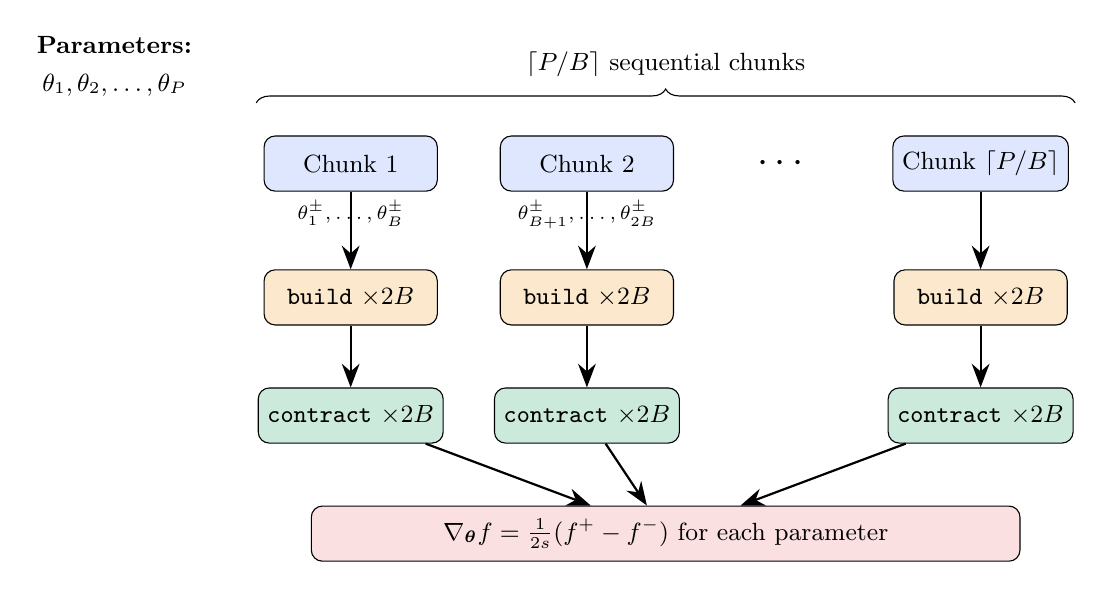
\begin{tikzpicture}[
    box/.style={draw, rounded corners, minimum width=2.2cm, minimum height=0.7cm, font=\small},
    arrow/.style={-{Stealth[length=3mm]}, thick},
    brace/.style={decorate, decoration={brace, amplitude=5pt, raise=2pt}}
]
% Parameters
\node[font=\small\bfseries] at (-3, 3) {Parameters:};
\node[font=\small] at (-3, 2.5) {$\theta_1, \theta_2, \ldots, \theta_P$};

% Chunk 1
\node[box, fill=trevblue!15] (c1) at (0, 1.5) {Chunk 1};
\node[font=\scriptsize, below=0pt of c1] {$\theta_{1}^{\pm}, \ldots, \theta_{B}^{\pm}$};

% Chunk 2
\node[box, fill=trevblue!15] (c2) at (3, 1.5) {Chunk 2};
\node[font=\scriptsize, below=0pt of c2] {$\theta_{B+1}^{\pm}, \ldots, \theta_{2B}^{\pm}$};

% Chunk k
\node[font=\Large] at (5.5, 1.5) {$\cdots$};

% Chunk last
\node[box, fill=trevblue!15] (ck) at (8, 1.5) {Chunk $\lceil P/B \rceil$};

% Build
\node[box, fill=trevorange!20] (b1) at (0, -0.2) {\texttt{build} $\times 2B$};
\node[box, fill=trevorange!20] (b2) at (3, -0.2) {\texttt{build} $\times 2B$};
\node[box, fill=trevorange!20] (bk) at (8, -0.2) {\texttt{build} $\times 2B$};

% Contract
\node[box, fill=trevgreen!20] (e1) at (0, -1.7) {\texttt{contract} $\times 2B$};
\node[box, fill=trevgreen!20] (e2) at (3, -1.7) {\texttt{contract} $\times 2B$};
\node[box, fill=trevgreen!20] (ek) at (8, -1.7) {\texttt{contract} $\times 2B$};

% Arrows
\draw[arrow] (c1) -- (b1);
\draw[arrow] (c2) -- (b2);
\draw[arrow] (ck) -- (bk);
\draw[arrow] (b1) -- (e1);
\draw[arrow] (b2) -- (e2);
\draw[arrow] (bk) -- (ek);

% Gradient
\node[box, fill=trevred!15, minimum width=9cm] (grad) at (4, -3.2) {$\nabla_{\boldsymbol{\theta}} f = \frac{1}{2s}(f^+ - f^-)$ for each parameter};
\draw[arrow] (e1) -- (grad);
\draw[arrow] (e2) -- (grad);
\draw[arrow] (ek) -- (grad);

% Annotation
\draw[brace] (-1.2, 2.2) -- (9.2, 2.2) node[midway, above=8pt, font=\small] {$\lceil P/B \rceil$ sequential chunks};

\end{tikzpicture}
\end{center}

\subsection{Cost Analysis}
\begin{itemize}
    \item \textbf{Number of chunks}: $\lceil P / B \rceil$ where $B$ = batch size (limited by GPU memory)
    \item \textbf{Per chunk}: Build $2B$ circuits + contract $2B \times T$ Hamiltonian terms
    \item \textbf{Total}: $\lceil P/B \rceil \times (2B \cdot C_{\text{build}} + 2B \cdot T \cdot N \cdot \chi^5)$
\end{itemize}

On a \textbf{large GPU} (A100, 40--80 GB): $B$ can equal $P$, so only $1$ chunk needed $\Rightarrow$ very fast.\\
On a \textbf{small GPU} (8 GB): $B \ll P$, many chunks $\Rightarrow$ slower.

%=============================================
\section{Autograd (Backpropagation)}

\subsection{Principle}
Build the circuit \textbf{once} with gradient tracking, compute the loss, then call \texttt{loss.backward()}. PyTorch's reverse-mode AD computes $\nabla_{\boldsymbol{\theta}} f$ in a \textbf{single backward pass}.

\begin{center}
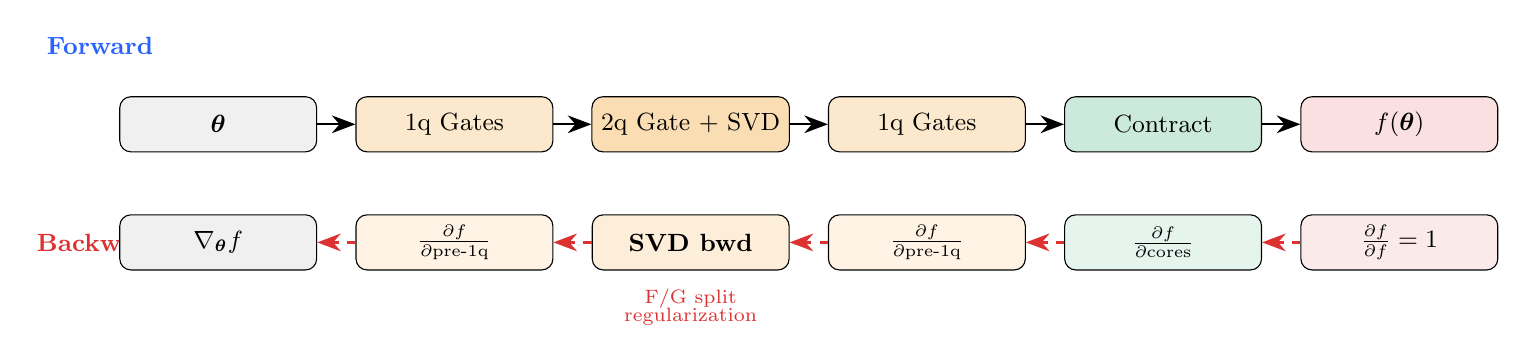
\begin{tikzpicture}[
    box/.style={draw, rounded corners, minimum width=2.5cm, minimum height=0.7cm, font=\small},
    arrow/.style={-{Stealth[length=3mm]}, thick},
    redarrow/.style={-{Stealth[length=3mm]}, thick, trevred, dashed}
]
% Forward pass
\node[font=\small\bfseries, trevblue] at (-1.5, 2) {Forward};

\node[box, fill=lightgray] (theta) at (0, 1) {$\boldsymbol{\theta}$};
\node[box, fill=trevorange!20] (gates) at (3, 1) {1q Gates};
\node[box, fill=trevorange!30] (svd) at (6, 1) {2q Gate + SVD};
\node[box, fill=trevorange!20] (gates2) at (9, 1) {1q Gates};
\node[box, fill=trevgreen!20] (contract) at (12, 1) {Contract};
\node[box, fill=trevred!15] (loss) at (15, 1) {$f(\boldsymbol{\theta})$};

\draw[arrow] (theta) -- (gates);
\draw[arrow] (gates) -- (svd);
\draw[arrow] (svd) -- (gates2);
\draw[arrow] (gates2) -- (contract);
\draw[arrow] (contract) -- (loss);

% Backward pass
\node[font=\small\bfseries, trevred] at (-1.5, -0.5) {Backward};

\node[box, fill=trevred!10] (dloss) at (15, -0.5) {$\frac{\partial f}{\partial f} = 1$};
\node[box, fill=trevgreen!10] (dcontract) at (12, -0.5) {$\frac{\partial f}{\partial \text{cores}}$};
\node[box, fill=trevorange!10] (dgates2) at (9, -0.5) {$\frac{\partial f}{\partial \text{pre-1q}}$};
\node[box, fill=trevorange!15] (dsvd) at (6, -0.5) {\textbf{SVD bwd}};
\node[box, fill=trevorange!10] (dgates) at (3, -0.5) {$\frac{\partial f}{\partial \text{pre-1q}}$};
\node[box, fill=lightgray] (dtheta) at (0, -0.5) {$\nabla_{\boldsymbol{\theta}} f$};

\draw[redarrow] (dloss) -- (dcontract);
\draw[redarrow] (dcontract) -- (dgates2);
\draw[redarrow] (dgates2) -- (dsvd);
\draw[redarrow] (dsvd) -- (dgates);
\draw[redarrow] (dgates) -- (dtheta);

% Annotations
\node[font=\scriptsize, text=trevred, below=3pt of dsvd] {F/G split};
\node[font=\scriptsize, text=trevred, below=10pt of dsvd] {regularization};

\end{tikzpicture}
\end{center}

\subsection{The SVD Backward Challenge}

The 2-qubit gate applies SVD to split the combined tensor:
\[
M = U \Sigma V^\dagger \quad \xrightarrow{\text{truncate}} \quad A_0' = U_k \Sigma_k, \quad A_1' = V_k^\dagger
\]

The backward through SVD requires computing $\partial A / \partial M$ given $\partial f / \partial U_k$, $\partial f / \partial \Sigma_k$, $\partial f / \partial V_k^\dagger$.

\textbf{Problem}: For complex matrices, the SVD has phase ambiguity ($U \to U \cdot \text{diag}(e^{i\phi})$), and the standard backward formula involves the ill-conditioned $F$ matrix:
\[
F_{ij} = \frac{1}{\sigma_j^2 - \sigma_i^2} \quad \xrightarrow{\sigma_i \approx \sigma_j} \quad \infty
\]

\textbf{Solution} (from Francuz et al.\ 2311.11894, peps-torch): Split $F$ into two well-conditioned terms:
\[
\frac{1}{\sigma_j^2 - \sigma_i^2} = \underbrace{\frac{1}{\sigma_j - \sigma_i}}_{\text{inv\_diff}} \cdot \underbrace{\frac{1}{\sigma_j + \sigma_i}}_{\text{inv\_sum}}
\]

When $\sigma_i \approx \sigma_j$: only inv\_diff is large, inv\_sum is well-behaved. Apply Lorentzian broadening to inv\_diff:
\[
\texttt{safe\_inv}(x) = \frac{x}{x^2 + \epsilon^2}
\]

The full backward formula:
\begin{align}
\mathcal{A} &= \frac{U^\dagger dU - dU^\dagger U}{2}, \quad \mathcal{B} = \frac{V^\dagger dV - dV^\dagger V}{2} \\
M_{\text{rot}} &= (\mathcal{A} + \mathcal{B}) \odot \texttt{inv\_diff} + (\mathcal{A} - \mathcal{B}) \odot \texttt{inv\_sum} \\
\frac{\partial f}{\partial A} &= U \left( M_{\text{rot}} + \text{diag}(d\Sigma) + \text{complex correction} \right) V^\dagger + \text{complement terms}
\end{align}

%=============================================
\section{Visual Comparison}

\begin{center}
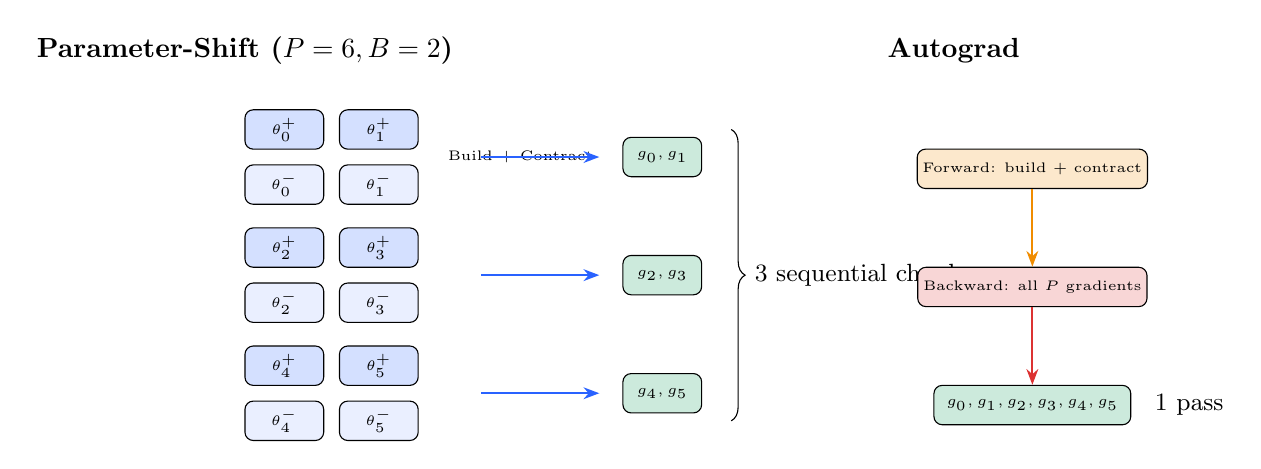
\begin{tikzpicture}[
    cbox/.style={draw, rounded corners=3pt, minimum width=1cm, minimum height=0.5cm, font=\tiny, inner sep=2pt},
    arrow/.style={-{Stealth[length=2mm]}, thick}
]

% === Parameter-Shift ===
\node[font=\bfseries] at (-0.5, 5.5) {Parameter-Shift ($P=6, B=2$)};

% Chunk 1
\foreach \i in {0,1} {
    \node[cbox, fill=trevblue!20] at (\i*1.2, 4.5) {$\theta_\i^+$};
    \node[cbox, fill=trevblue!10] at (\i*1.2, 3.8) {$\theta_\i^-$};
}
\node[font=\tiny] at (3, 4.15) {Build + Contract};
\draw[arrow, trevblue] (2.5, 4.15) -- (4, 4.15);
\node[cbox, fill=trevgreen!20] at (4.8, 4.15) {$g_0, g_1$};

% Chunk 2
\foreach \i in {2,3} {
    \pgfmathtruncatemacro{\x}{\i-2}
    \node[cbox, fill=trevblue!20] at (\x*1.2, 3) {$\theta_\i^+$};
    \node[cbox, fill=trevblue!10] at (\x*1.2, 2.3) {$\theta_\i^-$};
}
\draw[arrow, trevblue] (2.5, 2.65) -- (4, 2.65);
\node[cbox, fill=trevgreen!20] at (4.8, 2.65) {$g_2, g_3$};

% Chunk 3
\foreach \i in {4,5} {
    \pgfmathtruncatemacro{\x}{\i-4}
    \node[cbox, fill=trevblue!20] at (\x*1.2, 1.5) {$\theta_\i^+$};
    \node[cbox, fill=trevblue!10] at (\x*1.2, 0.8) {$\theta_\i^-$};
}
\draw[arrow, trevblue] (2.5, 1.15) -- (4, 1.15);
\node[cbox, fill=trevgreen!20] at (4.8, 1.15) {$g_4, g_5$};

\draw[decorate, decoration={brace, amplitude=5pt, mirror, raise=5pt}]
    (5.5, 0.8) -- (5.5, 4.5) node[midway, right=10pt, font=\small] {3 sequential chunks};

% === Autograd ===
\node[font=\bfseries] at (8.5, 5.5) {Autograd};

\node[cbox, fill=trevorange!20, minimum width=2.5cm] (fwd) at (9.5, 4) {Forward: build + contract};
\node[cbox, fill=trevred!20, minimum width=2.5cm] (bwd) at (9.5, 2.5) {Backward: all $P$ gradients};

\draw[arrow, trevorange] (fwd) -- (bwd);

\node[cbox, fill=trevgreen!20, minimum width=2.5cm] (grad) at (9.5, 1) {$g_0, g_1, g_2, g_3, g_4, g_5$};
\draw[arrow, trevred] (bwd) -- (grad);

\node[font=\small, right=5pt of grad] {1 pass};

\end{tikzpicture}
\end{center}

%=============================================
\section{When Each Method Wins}

\begin{center}
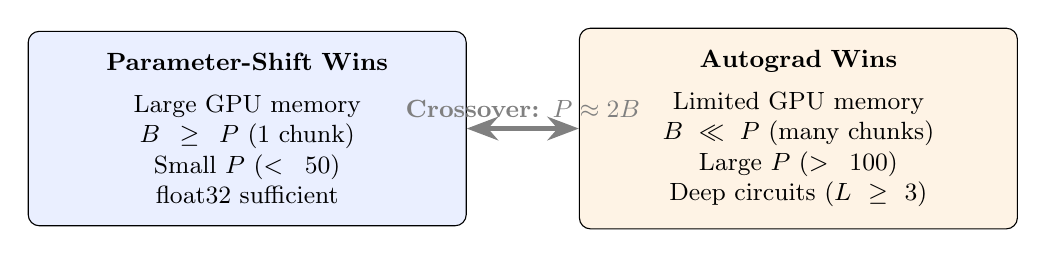
\begin{tikzpicture}[
    box/.style={draw, rounded corners, font=\small, text width=5cm, align=center, inner sep=8pt}
]
\node[box, fill=trevblue!10] (ps) at (0, 0) {
    \textbf{Parameter-Shift Wins}\\[4pt]
    Large GPU memory\\
    $B \geq P$ (1 chunk)\\
    Small $P$ ($< 50$)\\
    float32 sufficient
};

\node[box, fill=trevorange!10] (ad) at (7, 0) {
    \textbf{Autograd Wins}\\[4pt]
    Limited GPU memory\\
    $B \ll P$ (many chunks)\\
    Large $P$ ($> 100$)\\
    Deep circuits ($L \geq 3$)
};

\draw[{Stealth[length=4mm]}-{Stealth[length=4mm]}, ultra thick, gray]
    (ps.east) -- (ad.west) node[midway, above, font=\small\bfseries] {Crossover: $P \approx 2B$};

\end{tikzpicture}
\end{center}

\subsection{Cost Formulas}

\textbf{Parameter-shift:}
\[
C_{\text{PS}} = \left\lceil \frac{P}{B} \right\rceil \times 2B \times \left( C_{\text{build}}^{\text{f32}} + T \cdot N \cdot \chi^5 \right)
\]

\textbf{Autograd:}
\[
C_{\text{AD}} = \underbrace{C_{\text{build}}^{\text{f32}}}_{\text{forward}} + \underbrace{T \cdot N \cdot \chi^4}_{\text{contraction}} + \underbrace{\alpha \cdot (C_{\text{build}} + T \cdot N \cdot \chi^4)}_{\text{backward} (\alpha \approx 1.5)}
\]

The ratio:
\[
\frac{C_{\text{PS}}}{C_{\text{AD}}} \approx \frac{2P/B \cdot (C_{\text{build}} + T \cdot N \cdot \chi^5)}{(1 + \alpha) \cdot (C_{\text{build}} + T \cdot N \cdot \chi^4)}
\]

When $B = P$: ratio $\approx 2 / (1 + \alpha) \approx 0.8$ (param-shift wins).\\
When $B = 8, P = 64$: ratio $\approx 16 / 2.5 \approx 6.4$ (autograd wins).

%=============================================
\section{Benchmark Results}

\subsection{RTX 4070 (8 GB, $B = 8$)}
\begin{center}
\begin{tabular}{lccccc}
\toprule
Circuit & $P$ & Autograd & Param-Shift & Speedup & Accuracy \\
\midrule
$N=8, \chi=10, L=2$ & 32 & 113 ms & 192 ms & 1.7$\times$ & cos = 0.999 \\
$N=12, \chi=10, L=2$ & 48 & 184 ms & 352 ms & 1.9$\times$ & cos = 0.999 \\
$N=16, \chi=4, L=2$ & 64 & 200 ms & 677 ms & 3.4$\times$ & cos = 0.996 \\
\bottomrule
\end{tabular}
\end{center}

\subsection{A100 (40 GB, $B = P$)}
\begin{center}
\begin{tabular}{lccccc}
\toprule
Circuit & $P$ & Autograd & Param-Shift & Speedup \\
\midrule
$N=12, \chi=10, L=2$ & 48 & 355 ms & 192 ms & 0.54$\times$ \\
$N=16, \chi=10, L=3$ & 96 & 527 ms & 583 ms & 1.11$\times$ \\
$N=24, \chi=10, L=2$ & 96 & 732 ms & 687 ms & 0.94$\times$ \\
\bottomrule
\end{tabular}
\end{center}

On A100, autograd and param-shift are comparable. Autograd wins at $N=16, L=3$ where the circuit is deep.

\end{document}
